\documentclass[11pt, a4paper]{article}

\usepackage[a4paper, margin=2.5cm]{geometry}
\usepackage[italian]{babel}
% \usepackage{parskip}
% \usepackage{graphicx}
% \usepackage{float}
% \usepackage{array}
% \usepackage{changepage}
% \usepackage{longtable}
% \usepackage{caption}
% \captionsetup[table]{skip=0.5cm}
% \usepackage{ragged2e}
% \usepackage[T1]{fontenc}
% \usepackage{helvet}
% \renewcommand{\familydefault}{\sfdefault}

\title{Progetto di Laboratorio

Programmazione a Oggetti

a.a. 2025-2026}

\author{David Sirbu - Matricola: 2137981}

\begin{document}
\maketitle
\section{Introduzione}

L'obiettivo del seguente progetto è la realizzazione di
un'agenda per la gestione avanzata delle attività dell'utente.
Essa permette di gestire diversi tipi di attività, tra cui
impegni, scadenze e routine, ciascuna con le proprie
caratteristiche intrinseche, sia funzionali che di
visualizzazione grafica

Per la realizzazione dell'interfaccia, sono state prese come
modello applicazioni come Google Calendar e l'applicazione
Calendario presente su iOS, adattandole in modo da rendere
l'applicazione maggiormente funzionale su un ambiente desktop.

L'applicazione permette di gestire in modo intuitivo le diverse
tipologie di attività, evidenziandone sia le analogie che le
differenze. Oltre alle fondamentali funzionalità CRUD
(Create, Read, Update, Delete), sono presenti anche modi per
filtrare le attività in base alla preferenza dell'utente.
\section{Classi principali del modello logico}

\begin{figure}[H]
    \begin{adjustwidth}{-2cm}{-2cm}
        \centering
        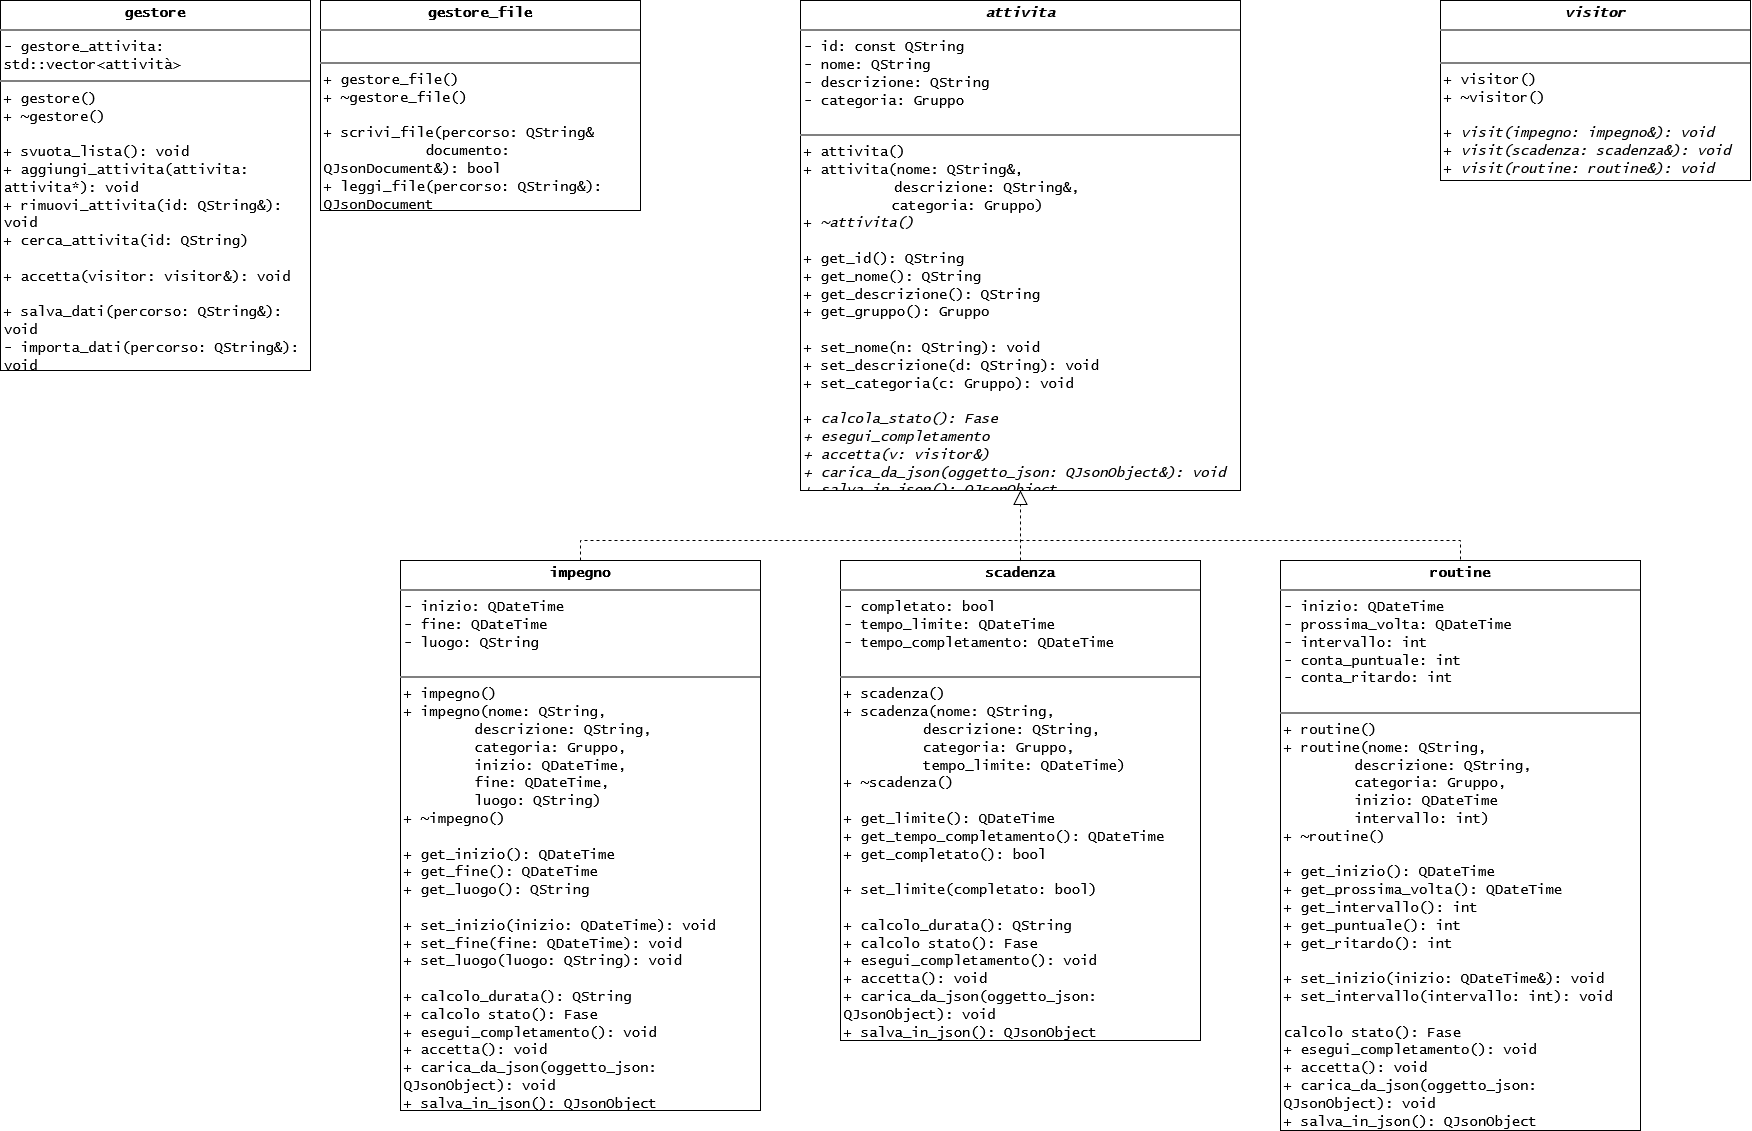
\includegraphics[width=1.25\textwidth, keepaspectratio]{allegati/uml_modello.drawio.png}
        \caption{Schema UML del modello logico}
        \label{fig:er-diagram}
    \end{adjustwidth}
\end{figure}

Per migliorare l'estensibilità del progetto, si è scelto di applicare
il design pattern architetturale MVC (Model-View-Controller), che
permette la separazione della logica dall'interfaccia grafica. In tale
contesto, la gestione delle caratteristiche funzionali delle attività è
affidata al Model.

Il fondamento dell'architettura è la classe base astratta \texttt{attivita}, che
presenta le caratteristiche base di ogni tipo di attività, come titolo, descrizione e
categoria di appartenenza.
Da essa derivano le classi concrete, cioè tipologie di attività con attributi strutturali
e comportamentali differenti tra loro. Attualmente, si è deciso di implementare le seguenti
categorie:
\begin{itemize}
    \item \textbf{Impegno}: caratterizzato da un inizio, una fine e il luogo in cui avviene.
    Non prevede un completamento, dato che si presuppone completato dopo la fine dell'impegno.
    \item \textbf{Scadenza}: non prevede un'inizio o una fine, ma solamente un limite e un
    tempo di completamento. Grazie a questi due elementi, diventa possibile tenere traccia
    dell'eventuale ritardo nel completamento della scadenza.
    \item \textbf{Routine}: non è caratterizzata da un tempo limite o di fine, ma è un'attività
    che si ripete indefinitamente. Impostando il tempo di inizio e l'intervallo, il sistema calcola
    automaticamente il termine della prossima iterazione della routine. Il sistema permette
    anche il numero di volte in cui è stata completata l'iterazione, tenendo anche traccia di
    puntualità e ritardi.
\end{itemize}

La gestione vera e propria delle instanze delle classi è affidata alla classe \texttt{gestore},
che, tramite un \texttt{std::vector<attivita*>} permette all'applicazione di effettuare le
operazioni CRUD. I vantaggi dell'uso di puntatori alla classe astratta \texttt{attivita} sono
la possibilità di implementare il polimorfismo e il rispetto del principio Open-Closed:
è possibile, infatti, inserire altre classi derivate concrete senza necessità di modificare
il codice del gestore.

Si è scelto di usare un \texttt{std::vector} per sfruttare la proprietà di continuità dei vettori:
infatti, le operazioni effettuate più frequentemente sono l'accesso arbitrario (visualizzazione e
modifica di un'attività) e l'accesso in serie (il refresh dell'intero elenco visivo in seguito a
modifiche o eliminazioni).

Il \texttt{gestore} contiene anche un \texttt{gestore\_file}, che si occupa esclusivamente della
persistenza delle attività.

Infine, il Model contiene la classe astratta \texttt{visitor}, da cui derivano i vari visitor usati
all'interno del programma per semplificare il codice grazie all'applicazione del polimorfismo.
\section{Utilizzo del polimorfismo}

In linea con la separazione imposta dal design pattern MVC, l'applicazione del polimorfismo
all'interno del progetto avviene in due fasi.

\subsection{Modello logico}

All'interno del modello logico, l'applicazione del polimorfismo si fonda sulla definizione di
alcune funzioni virtuali pure nella classe base astratta \texttt{attivita}.
Tali metodi forniscono un'interfaccia comune per caratteristiche trasversali ad ogni tipo di
attività (come la possibilità di essere completate), lasciando alle classi derivate l'implementazione
del comportamento specifico.
Il dominio di applicazione di queste funzioni è esclusivamente il \textbf{Model}, garantendone l'indipendenza
rispetto all'interfaccia grafica e permettendone il riutilizzo in altri contesti (cambio di framework
per l'interfaccia, passaggio da interfaccia grafica a client a linea di comando (CLI), ...).

\subsection{Design Pattern Visitor}

Per rendere la \textbf{View} il più passiva possibile rispetto ai dati in input, si è scelto di
affidare l'estrazione e la gestione dei dati grezzi al \textbf{Controller}. Alle classi
intermedie dell'interfaccia grafica viene affidato solamente il compito di inoltrare i pacchetti ricevuti
dal controller alle classi predisposte alla visualizzazione dei dati.
Per gestire i dati grezzi è stato deciso di utilizzare i DTO (Data Transfer Object), in modo da
slegare la logica delle classi dalla visualizzazione finale nell'interfaccia grafica.

L'applicazione del polimorfismo a questo processo avviene nel controller, grazie all'applicazione
del design pattern Visitor. Grazie al Double Dispatch (doppio smistamento), la classe concreta
restituisce il puntatore a se stessa \texttt{this}, invocando autonomamente la funzione corretta
del visitor.

In particolare, nel progetto i visitor sono stati usati per generare dinamicamente i DTO contenenti
i dettagli delle attività necessarie in un determinato momento all'interfaccia grafica.

Nel primo caso, ad ogni aggiornamento della schermata principale (che avviene ad ogni creazione, modifica
o eliminazione di un'attività, in modo da garantire la sincronizzazione tra \textit{Model} e
\textit{View}), il controller prende tutte le attività presenti nel \texttt{gestore}, ne genera il
DTO corrispondente e lo smista nella lista corretta, predisponendone la visualizzazione nella
schermata principale.

Invece, nel secondo caso, il visitor agisce su un'attività generica, identificata tramite ID
univoco, estraendone dinamicamente i dati grezzi e generando il rispettivo DTO, che successivamente
verrà inoltrato alla finestra richiedente (che sia essa di modifica o di visualizzazione dettagliata
in sola lettura).

Grazie all'applicazione del polimorfismo e del design pattern \textit{Visitor}, è possibile far
lavorare la classe \texttt{gestore} esclusivamente con puntatori ad attività generiche,
favorendo l'estensibilità del codice.
\section{Metodo di persistenza dei dati}

Per garantire la persistenza dei dati anche in seguito alla chiusura dell'applicazione, si è
scelto di utilizzare il formato JSON, data la presenza di classi apposite nel framework Qt, tra cui
\texttt{QJsonObject}, \texttt{QJsonArray}, \texttt{QJsonDocument}.

La gestione a basso livello del file (con nome di default \texttt{agenda.json}) viene affidata
alla classe \texttt{gestione\_file}, contenuta nella classe \texttt{gestore}.
Tramite i dati ricevuti, il \texttt{gestore} è in grado di ricostruire lo storico di tutte
le attività presenti all'ultimo salvataggio.

Il file è unico, e, al suo interno, le attività sono contenute in un array. In ogni attività
singola, i dati sono disposti in modalità chiave-valore. Tra queste coppie, ne è presente una
che identifica la tipologia di attività, usata dalla classe \texttt{gestore} per creare il
tipo di attività corretta. La coerenza dell'intero elenco di attività tra diverse esecuzioni
del programma viene garantita dalla presenza del campo ID in ogni attività.
\section{Funzionalità aggiuntive}

Le funzionalità implementate nell'applicazione si dividono in due categorie principali: logico-funzionali e di interfaccia grafica (GUI).

Tra le funzionalità logico-funzionali rientrano:
\begin{itemize}
    \item Gestione di tre tipologie di attività differenti;
    \item Salvataggio e caricamento dei dati in formato JSON;
    \item Calcolo automatico dello stato dell'attività (in corso, completata, scaduta, ecc.) con comportamento personalizzato in base alla tipologia;
    \item Calcolo automatico della durata per la categoria degli impegni.
\end{itemize}

Per quanto riguarda le funzionalità legate all'interfaccia grafica, sono state implementate:
\begin{itemize}
    \item Suddivisione visiva automatica delle attività nelle rispettive colonne;
    \item Visualizzazione dettagliata di un'attività tramite doppio click;
    \item Sistema di sicurezza con avviso di emergenza in caso di chiusura con modifiche non salvate;
    \item Scorciatoie da tastiera per le azioni principali (salvataggio, caricamento, creazione ed eliminazione);
    \item Barra di ricerca reattiva in tempo reale e \textit{case-insensitive};
    \item Gestione dinamica del ridimensionamento della finestra;
    \item Alternanza dei colori nelle liste (\textit{zebra striping}), per facilitare la lettura e la distinzione visiva degli elementi.
\end{itemize}
\section{Rendicontazione delle ore}

Questa sezione riporta le fasi affrontate nella realizzazione del progetto, insieme alla rendicontazione delle ore previste e di quelle effettivamente impiegate.

Per massimizzare la separazione imposta dall'architettura MVC, si è deciso di sviluppare l'intero motore logico prima dell'apprendimento del framework Qt. Fanno eccezione le classi \texttt{QString} e \texttt{QDateTime}, dato che non sono inerenti all'interfaccia grafica.

Per quanto riguarda la GUI, si è scelto di procedere con un approccio ``sul campo'': invece di imparare tutte le classi principali del framework, si è preferito suddividere lo sviluppo in micro-fasi: ad ognuna corrisponde una fase di apprendimento immediatamente seguita da quella di sviluppo.

\begin{table}[h!]
\centering
\renewcommand{\arraystretch}{1.3}
\begin{tabular}{|l|c|c|}
\hline
\textbf{Attività} & \textbf{Ore Previste} & \textbf{Ore Effettive} \\
\hline
Progettazione del modello & 3 & 2 \\
\hline
Sviluppo e test del modello & 4 & 3 \\
\hline
Studio e progettazione dello scheletro della GUI & 6 & 7 \\
\hline
Studio e implementazione del sistema \textit{Signals-Slots} & 6 & 8 \\
\hline
Test di segnali e slots (solo GUI) & 3 & 2 \\
\hline
Sviluppo del controller e connessione delle parti & 5 & 6 \\
\hline
Test e debug generale & 3 & 6 \\
\hline
Implementazione della persistenza & 3 & 2 \\
\hline
Aggiunta funzionalità extra & 2 & 3 \\
\hline
Test e debug finale & 2 & 3 \\
\hline
Stesura della relazione & 3 & 3 \\
\hline\hline
\textbf{Totale}  & \textbf{40} & \textbf{45} \\
\hline
\end{tabular}
\end{table}

Lo sforamento del monte ore totale, per quanto non eccessivo (pari al 12,5\% del monte ore previsto),
è stato causato da una leggera difficoltà di apprendimento dei concetti più ostici del framework
Qt, come il sistema \textit{Signals-Slots}, e dalla fase di test e debug in seguito alla connessione
dei componenti dell'architettura MVC.
\end{document}